\section*{Lecture 01: Introduction}
\addcontentsline{toc}{section}{Lecture 01: Introduction}

In the physical sense, the word `relativity' can be used to relate the measurement of one observer with that of another, for the same object/quantity. So using relativity, we can characterise the difference in the observations of two observers in two different frame of reference. \\[0.2cm]
Note that, physical laws should not matter based on who is observing (that is, physical laws are \textit{universal}), hence \underline{relativity} becomes very important when dealing with the resolution of conflicts.\\[0.2cm]
Let us consider two reference frames, and let $v$ be the relative velocity between the frames. 
\begin{figure}[H]
    \centering
    

\tikzset{every picture/.style={line width=0.75pt}} %set default line width to 0.75pt        

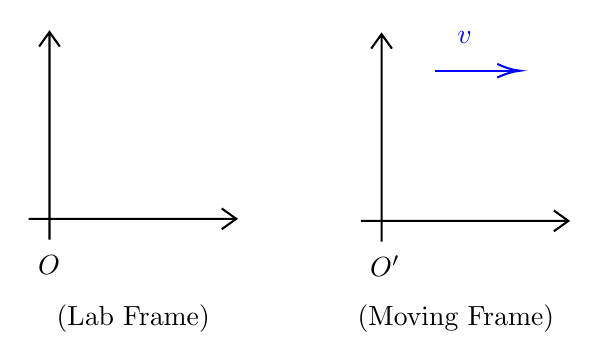
\begin{tikzpicture}[x=0.75pt,y=0.75pt,yscale=-1,xscale=1]
%uncomment if require: \path (0,193); %set diagram left start at 0, and has height of 193

%Shape: Axis 2D [id:dp9794610670096641] 
\draw  (171,118) -- (271,118)(181,28) -- (181,128) (264,113) -- (271,118) -- (264,123) (176,35) -- (181,28) -- (186,35)  ;
%Shape: Axis 2D [id:dp21159834766612584] 
\draw  (331,119) -- (431,119)(341,29) -- (341,129) (424,114) -- (431,119) -- (424,124) (336,36) -- (341,29) -- (346,36)  ;
%Straight Lines [id:da5217345963407499] 
\draw [color={rgb, 255:red, 0; green, 6; blue, 255 }  ,draw opacity=1 ]   (366.68,46.65) -- (405.68,46.65) ;
\draw [shift={(407.68,46.65)}, rotate = 180] [color={rgb, 255:red, 0; green, 6; blue, 255 }  ,draw opacity=1 ][line width=0.75]    (10.93,-3.29) .. controls (6.95,-1.4) and (3.31,-0.3) .. (0,0) .. controls (3.31,0.3) and (6.95,1.4) .. (10.93,3.29)   ;

% Text Node
\draw (376,26.4) node [anchor=north west][inner sep=0.75pt]  [color={rgb, 255:red, 0; green, 6; blue, 255 }  ,opacity=1 ]  {$v$};
% Text Node
\draw (174,134.4) node [anchor=north west][inner sep=0.75pt]    {$O$};
% Text Node
\draw (334,134.4) node [anchor=north west][inner sep=0.75pt]    {$O'$};
% Text Node
\draw (183,158) node [anchor=north west][inner sep=0.75pt]   [align=left] {(Lab Frame)};
% Text Node
\draw (328,158) node [anchor=north west][inner sep=0.75pt]   [align=left] {(Moving Frame)};


\end{tikzpicture}

    \caption{Two frames of reference with a relative velocity $v$}
    \label{fig:frame}
\end{figure}
\noindent
Fig. \ref{fig:frame} shows two reference frames. The moving frame is denoted by $O'$ (henceforth, primes will generally denote moving frames). If the relative velocity $v$ between the two frames remain constant, then it falls under the domain of \textit{Special Relativity} and if unfortunately (or fortunately) it doesn't, then it comes under \textit{General Relativity}. \\[0.2cm]

The theory of relativity dates back to the inception of Newtonian mechanics and hence, let us review the laws in brief (without being much technical \emoji{sweat-smile}):
\begin{itemize}
    \item \textbf{The First Law} $:\approx$ velocity of a body remains constant unless acted by an external, unbalanced force. 
    \item \textbf{The Second Law} $:\approx$ $\vec{F} = m\vec{a}$ where $\vec{F}$ is the external force and $\vec{a}$ is the acceleration. 
    \item \textbf{The Third Law} $:\approx$  Every action has an equal and opposite reaction. Note that for this, two bodies are needed.  
    \begin{figure}[H]
        \centering
        

\tikzset{every picture/.style={line width=0.75pt}} %set default line width to 0.75pt        

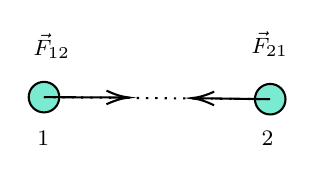
\begin{tikzpicture}[x=0.75pt,y=0.75pt,yscale=-1,xscale=1]
%uncomment if require: \path (0,137); %set diagram left start at 0, and has height of 137

%Shape: Circle [id:dp20820886588267196] 
\draw  [fill={rgb, 255:red, 80; green, 227; blue, 194 }  ,fill opacity=0.76 ] (259.28,82.36) .. controls (259.28,78.29) and (262.58,75) .. (266.64,75) .. controls (270.71,75) and (274,78.29) .. (274,82.36) .. controls (274,86.42) and (270.71,89.72) .. (266.64,89.72) .. controls (262.58,89.72) and (259.28,86.42) .. (259.28,82.36) -- cycle ;
%Shape: Circle [id:dp506083485076198] 
\draw  [fill={rgb, 255:red, 80; green, 227; blue, 194 }  ,fill opacity=0.76 ] (368.28,83.36) .. controls (368.28,79.29) and (371.58,76) .. (375.64,76) .. controls (379.71,76) and (383,79.29) .. (383,83.36) .. controls (383,87.42) and (379.71,90.72) .. (375.64,90.72) .. controls (371.58,90.72) and (368.28,87.42) .. (368.28,83.36) -- cycle ;
%Straight Lines [id:da6014834900744164] 
\draw    (266.64,82.36) -- (305.68,82.56) ;
\draw [shift={(307.68,82.57)}, rotate = 180.29] [color={rgb, 255:red, 0; green, 0; blue, 0 }  ][line width=0.75]    (10.93,-3.29) .. controls (6.95,-1.4) and (3.31,-0.3) .. (0,0) .. controls (3.31,0.3) and (6.95,1.4) .. (10.93,3.29)   ;
%Straight Lines [id:da5401751978276785] 
\draw    (375.64,83.36) -- (339.68,82.88) ;
\draw [shift={(337.68,82.85)}, rotate = 0.77] [color={rgb, 255:red, 0; green, 0; blue, 0 }  ][line width=0.75]    (10.93,-3.29) .. controls (6.95,-1.4) and (3.31,-0.3) .. (0,0) .. controls (3.31,0.3) and (6.95,1.4) .. (10.93,3.29)   ;
%Straight Lines [id:da23091707334387013] 
\draw  [dash pattern={on 0.84pt off 2.51pt}]  (266.64,82.36) -- (375.64,83.36) ;

% Text Node
\draw (260,50.4) node [anchor=north west][inner sep=0.75pt]  [font=\footnotesize]  {$\vec{F}_{12}$};
% Text Node
\draw (365,49.4) node [anchor=north west][inner sep=0.75pt]  [font=\footnotesize]  {$\vec{F}_{21}$};
% Text Node
\draw (262,97.4) node [anchor=north west][inner sep=0.75pt]  [font=\footnotesize]  {$1$};
% Text Node
\draw (370,97.4) node [anchor=north west][inner sep=0.75pt]  [font=\footnotesize]  {$2$};


\end{tikzpicture}

    \end{figure}
    From the figure above, we will have $\vec{F}_{21} = -\vec{F}_{12}$
    \item \textbf{The Gravitational Law} $:\approx$ 
    \begin{figure}[H]
        \centering 
        

\tikzset{every picture/.style={line width=0.75pt}} %set default line width to 0.75pt        

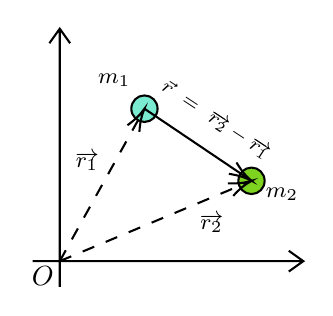
\begin{tikzpicture}[x=0.75pt,y=0.75pt,yscale=-1,xscale=1]
%uncomment if require: \path (0,178); %set diagram left start at 0, and has height of 178

%Shape: Axis 2D [id:dp42543499801858453] 
\draw  (222.72,138.99) -- (353.11,138.99)(235.76,27) -- (235.76,151.44) (346.11,133.99) -- (353.11,138.99) -- (346.11,143.99) (230.76,34) -- (235.76,27) -- (240.76,34)  ;
%Shape: Ellipse [id:dp34665186673267967] 
\draw  [fill={rgb, 255:red, 80; green, 227; blue, 194 }  ,fill opacity=0.76 ] (270.24,65.54) .. controls (270.24,62.01) and (273.08,59.14) .. (276.57,59.14) .. controls (280.06,59.14) and (282.89,62.01) .. (282.89,65.54) .. controls (282.89,69.07) and (280.06,71.93) .. (276.57,71.93) .. controls (273.08,71.93) and (270.24,69.07) .. (270.24,65.54) -- cycle ;
%Shape: Ellipse [id:dp9968570486343863] 
\draw  [fill={rgb, 255:red, 126; green, 211; blue, 33 }  ,fill opacity=1 ] (321.82,100.29) .. controls (321.82,96.76) and (324.65,93.9) .. (328.15,93.9) .. controls (331.64,93.9) and (334.47,96.76) .. (334.47,100.29) .. controls (334.47,103.82) and (331.64,106.68) .. (328.15,106.68) .. controls (324.65,106.68) and (321.82,103.82) .. (321.82,100.29) -- cycle ;
%Straight Lines [id:da8232147057285761] 
\draw  [dash pattern={on 4.5pt off 4.5pt}]  (235.76,138.99) -- (275.6,67.29) ;
\draw [shift={(276.57,65.54)}, rotate = 119.06] [color={rgb, 255:red, 0; green, 0; blue, 0 }  ][line width=0.75]    (10.93,-3.29) .. controls (6.95,-1.4) and (3.31,-0.3) .. (0,0) .. controls (3.31,0.3) and (6.95,1.4) .. (10.93,3.29)   ;
%Straight Lines [id:da9672340288452689] 
\draw  [dash pattern={on 4.5pt off 4.5pt}]  (235.76,138.99) -- (326.3,101.06) ;
\draw [shift={(328.15,100.29)}, rotate = 157.27] [color={rgb, 255:red, 0; green, 0; blue, 0 }  ][line width=0.75]    (10.93,-3.29) .. controls (6.95,-1.4) and (3.31,-0.3) .. (0,0) .. controls (3.31,0.3) and (6.95,1.4) .. (10.93,3.29)   ;
%Straight Lines [id:da6937866085380056] 
\draw    (276.57,65.54) -- (326.49,99.17) ;
\draw [shift={(328.15,100.29)}, rotate = 213.97] [color={rgb, 255:red, 0; green, 0; blue, 0 }  ][line width=0.75]    (10.93,-3.29) .. controls (6.95,-1.4) and (3.31,-0.3) .. (0,0) .. controls (3.31,0.3) and (6.95,1.4) .. (10.93,3.29)   ;

% Text Node
\draw (241.74,85.16) node [anchor=north west][inner sep=0.75pt]  [font=\footnotesize]  {$\overrightarrow{r_{1}}$};
% Text Node
\draw (301.74,114.97) node [anchor=north west][inner sep=0.75pt]  [font=\footnotesize]  {$\overrightarrow{r_{2}}$};
% Text Node
\draw (287.5,48.56) node [anchor=north west][inner sep=0.75pt]  [font=\scriptsize,rotate=-33.42]  {$\vec{r} \ =\ \overrightarrow{r_{2}} -\overrightarrow{r_{1}}$};
% Text Node
\draw (220.81,140.09) node [anchor=north west][inner sep=0.75pt]    {$O$};
% Text Node
\draw (252.77,47.33) node [anchor=north west][inner sep=0.75pt]  [font=\footnotesize]  {$m_{1}{}$};
% Text Node
\draw (333.58,102.38) node [anchor=north west][inner sep=0.75pt]  [font=\footnotesize]  {$m_{2}{}$};


\end{tikzpicture}

    \end{figure}
    \noindent
    In the above situation, if we consider for mass $m_1$, we have:
     $$\vec{F}_{12} = G \frac{m_1 m_2}{\rcurs_{21}^2}\hat{\rcurs_{21}}$$
\end{itemize}
\noindent
An important observation: in the second law, if we take the force to be zero, then apparently $\vec{a}= \dv{v}{t} = 0\implies \vec{v} = \mathrm{const.}$ which is the statement of the first law. However, the second law does not imply the first law, since the first law defines what an \textit{inertial frame} is and the statement of the second law applies only in case of inertial frames. So, a better formulation of the second and third law can be like, ``In a frame where the first law is valid, blah blah blah...''